
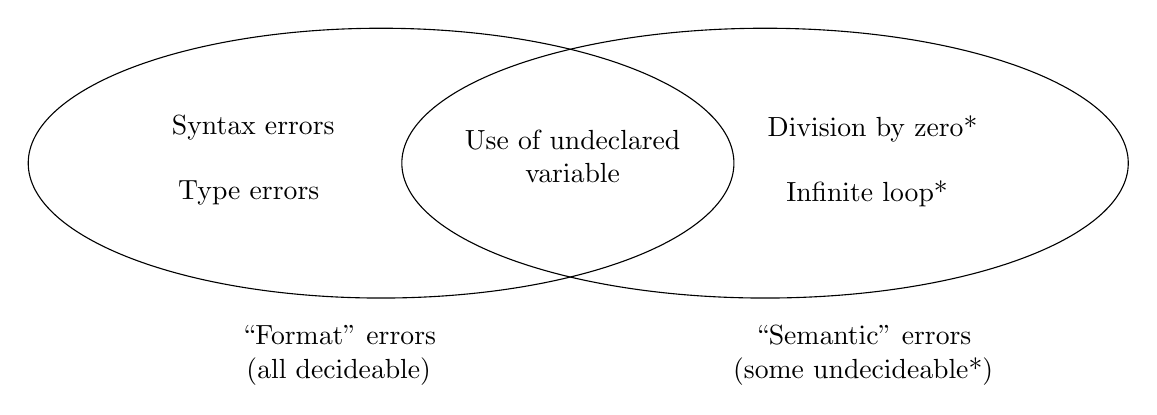
\begin{tikzpicture}[x=0.75pt,y=0.75pt,yscale=-1,xscale=1]
%uncomment if require: \path (0,300); %set diagram left start at 0, and has height of 300

%Shape: Ellipse [id:dp5326335354678456] 
\draw   (210,85) .. controls (210,49.1) and (288.35,20) .. (385,20) .. controls (481.65,20) and (560,49.1) .. (560,85) .. controls (560,120.9) and (481.65,150) .. (385,150) .. controls (288.35,150) and (210,120.9) .. (210,85) -- cycle ;
%Shape: Ellipse [id:dp904564307478004] 
\draw   (30,85) .. controls (30,49.1) and (106.11,20) .. (200,20) .. controls (293.89,20) and (370,49.1) .. (370,85) .. controls (370,120.9) and (293.89,150) .. (200,150) .. controls (106.11,150) and (30,120.9) .. (30,85) -- cycle ;

% Text Node
\draw (98,61) node [anchor=north west][inner sep=0.75pt]   [align=left] {Syntax errors};
% Text Node
\draw (351,162) node [anchor=north west][inner sep=0.75pt]   [align=left] {\begin{minipage}[lt]{120pt}\setlength\topsep{0pt}
\begin{center}
“Semantic" errors\\(some undecideable*)
\end{center}

\end{minipage}};
% Text Node
\draw (125,162) node [anchor=north west][inner sep=0.75pt]   [align=left] {\begin{minipage}[lt]{80pt}\setlength\topsep{0pt}
\begin{center}
“Format" errors\\(all decideable)
\end{center}

\end{minipage}};
% Text Node
\draw (101,92) node [anchor=north west][inner sep=0.75pt]   [align=left] {Type errors};
% Text Node
\draw (231,68) node [anchor=north west][inner sep=0.75pt]   [align=left] {\begin{minipage}[lt]{90pt}\setlength\topsep{0pt}
\begin{center}
Use of undeclared\\variable
\end{center}

\end{minipage}};
% Text Node
\draw (385,61) node [anchor=north west][inner sep=0.75pt]   [align=left] {Division by zero*};
% Text Node
\draw (394,92) node [anchor=north west][inner sep=0.75pt]   [align=left] {Infinite loop*};


\end{tikzpicture}
